\documentclass[11pt,a4paper]{article}
\usepackage[margin=2cm]{geometry}
\usepackage[T1]{fontenc}
\usepackage[utf8]{inputenc}
\usepackage{lmodern,microtype}
\usepackage{amsmath,amssymb,mathtools,bm}
\usepackage{booktabs,tabularx,longtable,array,multirow}
\usepackage{graphicx,caption,subcaption,float}
\usepackage{enumitem,xcolor,hyperref,cleveref}
\usepackage{fancyhdr,titlesec,siunitx,url}
\usepackage[most]{tcolorbox}
\usepackage{tikz}
\usetikzlibrary{arrows.meta,positioning,fit,calc,shapes.geometric,backgrounds}

\definecolor{deepblue}{RGB}{28,63,105}
\definecolor{deepgreen}{RGB}{38,105,79}
\definecolor{deeporange}{RGB}{170,92,20}
\definecolor{deepred}{RGB}{145,52,52}
\definecolor{softblue}{RGB}{232,241,250}
\definecolor{softgreen}{RGB}{235,247,240}
\definecolor{softorange}{RGB}{253,243,226}
\definecolor{softred}{RGB}{252,235,235}
\definecolor{softgray}{RGB}{245,246,248}
\hypersetup{
 colorlinks=true,
 linkcolor=deepblue,
 citecolor=deepgreen,
 urlcolor=deeporange,
 pdftitle={Geometry-MMALS G1 v1.1.1: Bridge Isolation Results},
 pdfauthor={Guillaume Harbonnier}
}
\pagestyle{fancy}\fancyhf{}
\lhead{Geometry-MMALS G1}
\rhead{v1.1.1 bridge-isolation results}
\cfoot{\thepage}
\setlength{\headheight}{14pt}
\titleformat{\section}{\Large\bfseries\color{deepblue}}{\thesection}{0.8em}{}
\titleformat{\subsection}{\large\bfseries\color{deepgreen}}{\thesubsection}{0.8em}{}
\titleformat{\subsubsection}{\normalsize\bfseries\color{deeporange}}{\thesubsubsection}{0.8em}{}
\setlist[itemize]{leftmargin=1.5em,itemsep=2pt,topsep=3pt}
\setlist[enumerate]{leftmargin=1.7em,itemsep=3pt,topsep=3pt}
\renewcommand{\arraystretch}{1.14}
\newcolumntype{Y}{>{\raggedright\arraybackslash}X}
\newcolumntype{C}{>{\centering\arraybackslash}X}
\newcommand{\MMALS}{\textsc{MMALS}}
\newcommand{\R}{\mathbb{R}}
\newcommand{\E}{\mathbb{E}}
\newcommand{\loss}{\mathcal{L}}
\newcommand{\norm}[1]{\left\lVert #1 \right\rVert}
\newcommand{\softmax}{\operatorname{softmax}}
\newcommand{\KL}{\operatorname{KL}}
\newcommand{\OT}{\operatorname{OT}}
\newtcolorbox{plainbox}[1][]{title={#1},colback=softblue,colframe=deepblue!45,boxrule=.6pt,arc=2pt,left=8pt,right=8pt,top=7pt,bottom=7pt}
\newtcolorbox{positivebox}[1][]{title={#1},colback=softgreen,colframe=deepgreen!45,boxrule=.6pt,arc=2pt,left=8pt,right=8pt,top=7pt,bottom=7pt}
\newtcolorbox{warningbox}[1][]{title={#1},colback=softorange,colframe=deeporange!50,boxrule=.6pt,arc=2pt,left=8pt,right=8pt,top=7pt,bottom=7pt}
\newtcolorbox{criticalbox}[1][]{title={#1},colback=softred,colframe=deepred!50,boxrule=.6pt,arc=2pt,left=8pt,right=8pt,top=7pt,bottom=7pt}
\newtcolorbox{mathbox}[1][]{title={#1},colback=softgray,colframe=black!30,boxrule=.5pt,arc=1pt,left=8pt,right=8pt,top=7pt,bottom=7pt}

\begin{document}
\begin{titlepage}
\centering
\vspace*{0.45cm}
{\Huge\bfseries\color{deepblue} Geometry-MMALS G1 v1.1.1\par}
\vspace{0.25cm}
{\LARGE Bridge Isolation with a Common Host Bank\par}
\vspace{0.08cm}
{\LARGE and Common Functional Metric\par}
\vspace{0.4cm}
{\Large Five-seed results, corrected manifests, falsification outcome, and reviewer-facing interpretation\par}
\vspace{0.7cm}
{\Large Guillaume Harbonnier\par}
\vspace{0.15cm}
{\normalsize Independent MMALS research program\par}
\vspace{0.15cm}
{\normalsize \href{https://github.com/gharbonnier78/geometry-mmalls-g1}{github.com/gharbonnier78/geometry-mmalls-g1}\par}
\vspace{0.55cm}
{\normalsize RotatedMNIST pilot, five matched-compute seeds, June 2026\par}
\vfill
\begin{minipage}{0.94\textwidth}\small
\textbf{Epistemic status.} This report describes a completed five-seed pilot. The protocol-integrity gates passed: the sensory encoder, context encoder, common host bank, synthesis layer, classifier, and functional host-cost matrix were shared across router treatments, and router compute was matched. The preregistered hybrid-router qualification did not pass. Held-out nominal and functional distance-order effects were positive on average but had seed intervals crossing zero; local continuity, causal specificity, and operational non-degradation failed. Route-swap ordering and prediction-identity preservation passed. The result supports non-arbitrary functional structure in the frozen routing ecosystem, but not a qualified context-to-function bridge or an operationally superior router.
\end{minipage}
\vfill
\end{titlepage}

\begin{abstract}
Geometry-MMALS studies whether an inferred context geometry can organize routing through a modular host ecosystem in a way that is measurable, functionally meaningful, and useful under continual learning. Version 1.1.1 removes the principal confound of the preceding experiment: for each model seed, all router treatments share the same frozen sensory encoder, four-dimensional context encoder, host bank, synthesis normalization, classifier, and host-functional cost matrix. Only the router changes. We compare a 4,740-parameter MLP router (R0), a 20-parameter linear router (R1), a 24-parameter prototype-energy router (R2), and a 42-parameter hybrid directional-prototype energy router (R3) over five matched-compute seeds.

The preregistered R3-versus-R0 held-out effects are positive but non-qualifying: nominal distance-order correlation changes by $+0.0299$ with 95\% seed interval $[-0.0127,0.0725]$, and common-cost functional optimal-transport correlation changes by $+0.0218$ with interval $[-0.0148,0.0584]$. Prototype-based routers nevertheless reduce held-out functional stress: R2 changes stress by $-0.0502$ with interval $[-0.0592,-0.0412]$, and R3 by $-0.0416$ with interval $[-0.0624,-0.0208]$. This structural improvement is offset by severe local sensitivity: held-out functional continuity q95 is $1.945$ for R3 and $1.718$ for R2, compared with $0.344$ for R0 and $0.271$ for R1. The route-swap-order gate passes: far-factor swaps produce larger functional changes than near-factor swaps for all five R3 seeds. Causal specificity fails, with mean R3 functional CSR $0.897$ and only one of five seeds having a lower source-bootstrap bound above one. R3 loses $1.03$ percentage points of held-out accuracy and $1.99$ points of final trained accuracy relative to R0, although forgetting decreases by $0.14$ points.

The five-seed result therefore falsifies the current hybrid-router qualification while preserving a narrower finding: fixed routes encode non-arbitrary functional relations, but prototype-dominated energy routing is too sharp and not sufficiently causally aligned. We recommend a continuity-controlled simplex-residual router as the immediate next experiment before covariance/SPD geometry, memory transport, or adaptive host feedback.
\end{abstract}

\tableofcontents
\clearpage

\section{Reviewer decision summary}
\begin{criticalbox}[Primary decision]
\textbf{The v1.1.1 hybrid directional-prototype router does not qualify.} The experiment is not a failed execution: it is a successful isolation protocol that returns a negative architecture result. The common-bank design removes host co-adaptation as an explanation, making the negative evidence more informative than the partially positive v1.1.0 result.
\end{criticalbox}

\begin{positivebox}[What survives]
Two findings survive the stricter protocol. First, the frozen context and host ecosystem are numerically identical across treatments, so router comparisons are causally cleaner. Second, far route swaps produce larger common-cost functional changes than near route swaps. The fixed ecosystem therefore contains non-arbitrary route-function structure even though the tested hybrid router does not exploit it smoothly or operationally.
\end{positivebox}

\begin{table}[H]
\centering
\caption{Reviewer-facing gate outcome. ``Fail'' means that the preregistered threshold was not met; it does not imply a software or protocol failure.}
\label{tab:gates}
\small
\begin{tabularx}{\textwidth}{@{}Y c Y@{}}
\toprule
Gate & Outcome & Interpretation \\
\midrule
Context and common host bank frozen & Pass & Exact zero context and host-output deltas across treatments. \\
Equal router compute & Pass & 15,360 forward images and 80 optimizer steps per method and seed. \\
Held-out nominal mediation & Fail & R3--R0 mean positive; seed interval crosses zero. \\
Held-out functional mediation, common cost & Fail & R3--R0 mean positive; seed interval crosses zero. \\
Local continuity tail & Fail & Prototype-based route maps have much larger q95 sensitivity. \\
Route-swap order & Pass & Far swaps exceed near swaps in all five R3 seeds. \\
Functional causal specificity & Fail & Only one of five R3 seeds has lower CSR bound above one. \\
Prediction identity preservation & Pass & Small controlled interventions generally preserve the predicted class. \\
Operational non-degradation & Fail & Accuracy loss exceeds the preregistered one-point margin. \\
Mature host specialization & Not tested & Hosts were intentionally frozen; only allocation specificity was measured. \\
Memory transport & Not implemented & Deferred to a later stage. \\
Operational superiority & Not claimed & Not preregistered as a primary claim. \\
\bottomrule
\end{tabularx}
\end{table}


\subsection{Post-execution manifest correction}
The notebook completed all five model seeds and exported the numerical evidence,
but its original \texttt{claim\_manifest.json} retained a stale pre-execution
status string. The release package corrects the claim and run manifests to
\texttt{five\_seed\_pilot\_completed}. This is a metadata-only correction:
no CSV value, checkpoint hash, common-cost matrix, dense trace, figure, or gate
outcome was changed. The corrected primary decision is
\texttt{r3\_hybrid\_router\_not\_qualified}.

\section{Scientific question and isolation design}
\subsection{From route geometry to functional geometry}
Earlier MMALS prototypes established the key non-implication
\begin{equation}
 r_{\mathrm{current}}\approx r_{\mathrm{teacher}}
 \;\not\Rightarrow\;
 z_{M,\mathrm{current}}\approx z_{M,\mathrm{teacher}},
\end{equation}
because host representations, host transformations, and readouts can drift while route coefficients remain similar. The relevant object is therefore not only a route vector, but a route interpreted through host function. This motivates a cost-aware geometry over the route simplex rather than an unconstrained Euclidean treatment of routing coefficients.

Version 1.1.0 partially transmitted context order into route order, but each router trained a different host bank and therefore induced a different functional cost matrix. Version 1.1.1 asks a stricter question:
\begin{quote}
Given the same context map, the same fixed host functions, and the same functional cost matrix, does a constrained router produce more ordered, continuous, causally specific, and operationally safe allocation than a flexible MLP router?
\end{quote}

\subsection{The isolated causal chain}
\begin{figure}[H]
\centering
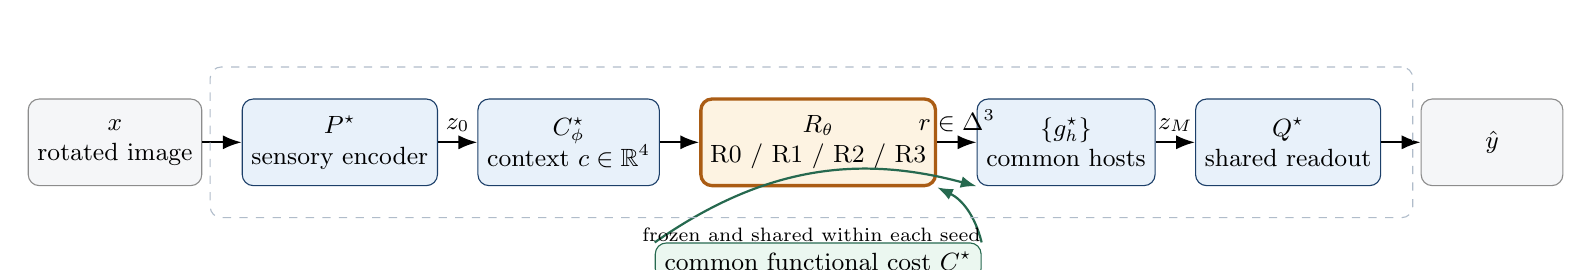
\begin{tikzpicture}[
 node distance=5mm and 5mm,
 every node/.style={font=\small,align=center},
 frozen/.style={draw=deepblue,fill=softblue,rounded corners,minimum height=11mm,minimum width=22mm},
 trainable/.style={draw=deeporange,fill=softorange,rounded corners,minimum height=11mm,minimum width=27mm,very thick},
 data/.style={draw=black!45,fill=softgray,rounded corners,minimum height=11mm,minimum width=18mm},
 arrow/.style={-{Latex[length=2.4mm]},thick}
]
\node[data] (x) {$x$\\rotated image};
\node[frozen,right=of x] (p) {$P^\star$\\sensory encoder};
\node[frozen,right=of p] (c) {$C_\phi^\star$\\context $c\in\R^4$};
\node[trainable,right=of c] (r) {$R_\theta$\\R0 / R1 / R2 / R3};
\node[frozen,right=of r] (h) {$\{g_h^\star\}$\\common hosts};
\node[frozen,right=of h] (q) {$Q^\star$\\shared readout};
\node[data,right=of q] (y) {$\hat y$};
\draw[arrow] (x)--(p);
\draw[arrow] (p)--node[above]{$z_0$}(c);
\draw[arrow] (c)--(r);
\draw[arrow] (r)--node[above]{$r\in\Delta^3$}(h);
\draw[arrow] (h)--node[above]{$z_M$}(q);
\draw[arrow] (q)--(y);
\node[below=7mm of r,draw=deepgreen,fill=softgreen,rounded corners,minimum width=38mm] (cost) {common functional cost $C^\star$};
\draw[-{Latex[length=2mm]},deepgreen,thick] (cost.north west) to[bend left=25] (h.south west);
\draw[-{Latex[length=2mm]},deepgreen,thick] (cost.north east) to[bend right=25] (r.south east);
\node[fit=(p)(c)(h)(q),draw=deepblue!35,dashed,rounded corners,inner sep=4mm,label=below:{\scriptsize frozen and shared within each seed}] {};
\end{tikzpicture}
\caption{v1.1.1 bridge isolation. Only the router is trainable during the treatment comparison. The host-functional cost matrix is built once from the common frozen host bank.}
\label{fig:architecture}
\end{figure}

\subsection{Routes still live on a probability simplex}
For four hosts, every routing vector satisfies
\begin{equation}
 r=(r_1,r_2,r_3,r_4)\in\Delta^3,
 \qquad r_h\ge 0,
 \qquad \sum_{h=1}^{4}r_h=1.
\end{equation}
The natural square-root embedding
\begin{equation}
 q(r)=\sqrt r
\end{equation}
maps the simplex to the positive orthant of the unit sphere. The nominal route distance used in the experiment is the root-simplex chord, equivalent to the Hellinger metric up to scale:
\begin{equation}
 d_R(r_a,r_b)=\frac{\norm{\sqrt{r_a}-\sqrt{r_b}}_2}{\sqrt 2}.
\end{equation}
This is not an unconstrained Euclidean distance between logits. It respects the probability budget and remains finite at sparse routes. A complementary Fisher--Rao distance could be tested later:
\begin{equation}
 d_{\mathrm{FR}}(r_a,r_b)=2\arccos\!\left(\sum_h\sqrt{r_{a,h}r_{b,h}}\right).
\end{equation}

\begin{figure}[H]
\centering
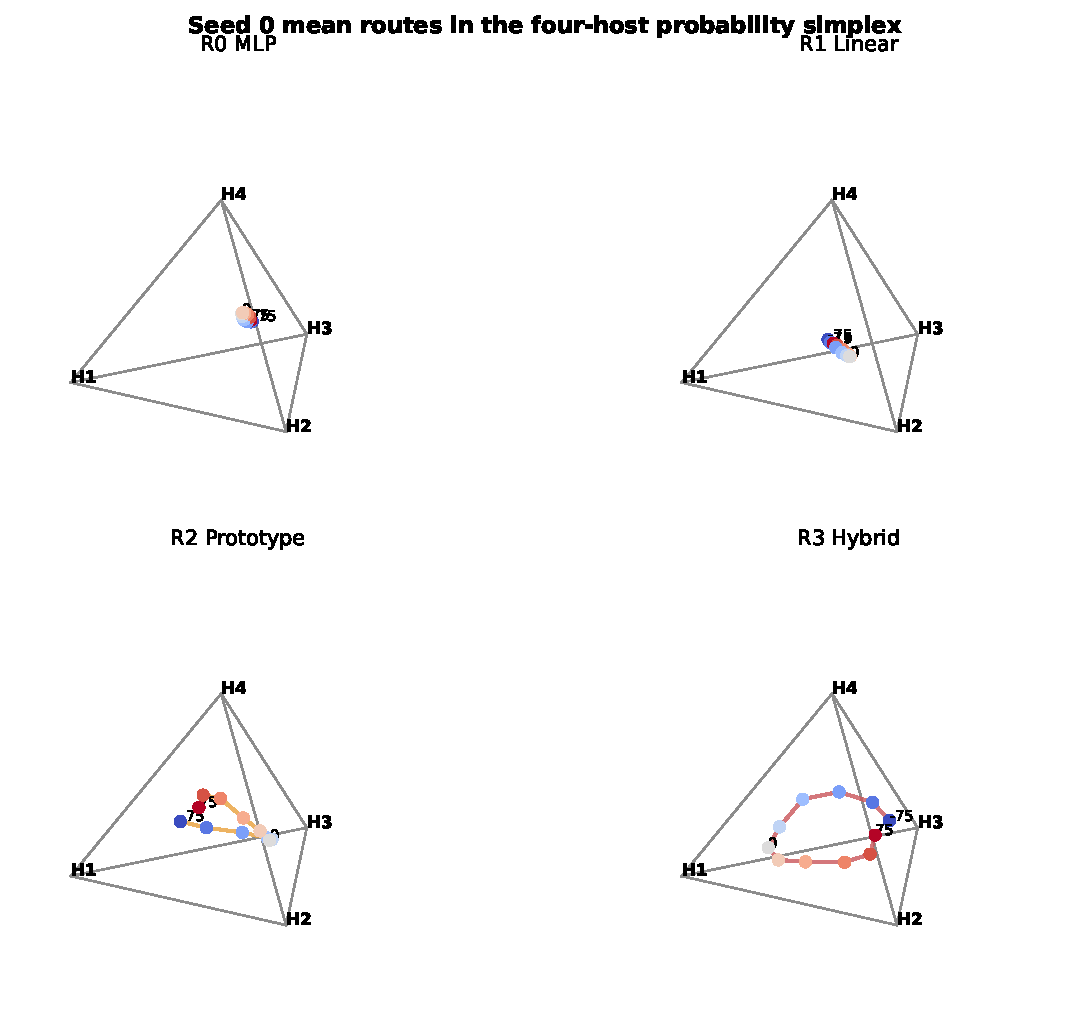
\includegraphics[width=0.92\textwidth]{figures/simplex_trajectories_seed0.pdf}
\caption{Seed-0 mean route trajectories on the four-host simplex. R0 and R1 remain comparatively smooth and diffuse. R2 and R3 create stronger territories and larger local movements. Labels mark $-75^\circ$, $0^\circ$, and $75^\circ$. This figure is descriptive; gates are computed from all sources and all five seeds.}
\label{fig:simplex}
\end{figure}

\section{Methods}
\subsection{Data and continual protocol}
The pilot uses RotatedMNIST. The continual curriculum is
\begin{equation}
 -60^\circ\rightarrow -30^\circ\rightarrow 0^\circ\rightarrow 60^\circ\rightarrow 30^\circ.
\end{equation}
The dense evaluation grid is
\begin{equation}
 \{-75,-60,-45,-30,-15,0,15,30,45,60,75\}^\circ,
\end{equation}
with six held-out factor values $\{-75,-45,-15,15,45,75\}^\circ$. The pilot uses 512 training source identities, 640 test identities, two epochs per stage, and model seeds $\{0,1,2,3,4\}$. Test identities are split into disjoint partitions for cost construction, mediation-probe fitting, mediation-probe evaluation, tangent fitting, causal evaluation, and route-swap evaluation.

\subsection{Common host bank}
A parameter-free uniform router
\begin{equation}
 r_h=\frac{1}{H}
\end{equation}
constructs one neutral bank per seed. The bank is trained with classification, retention anchoring, and weak host-output diversity, but without factor labels in routing. After this phase, the host bank, synthesis normalization, and classifier are frozen and copied into every treatment.

The shared host-functional cost is
\begin{equation}
 C^\star_{hk}=\E_x\left[\frac{\norm{g_h^\star(z_0(x))-g_k^\star(z_0(x))}_2^2}{d_M}\right],
\end{equation}
symmetrized, zeroed on the diagonal, and normalized by the median non-zero cost.

\subsection{Router treatments}
The four treatment families are:
\begin{align}
R_0(c)&=\softmax\!\left(W_2\phi(W_1c+b_1)+b_2\right),\\
R_1(c)&=\softmax(Wc+b),\\
E^{(2)}_h(c)&=\frac{d_C(c,\mu_h)^2}{2\sigma_h^2}+b_h,\\
E^{(3)}_h(c)&=\alpha\frac{d_C(c,\mu_h)^2}{2\sigma_h^2}-\beta a_h^\top c+b_h,\\
R_{k,h}(c)&=\frac{\exp[-E^{(k)}_h(c)/\tau]}{\sum_j\exp[-E^{(k)}_j(c)/\tau]},\quad k\in\{2,3\}.
\end{align}
R0 has 4,740 trainable parameters, R1 has 20, R2 has 24, and R3 has 42. R2 and R3 prototypes are initialized by spherical $k$-means without angle labels.

The router-only objective is
\begin{equation}
 \loss=\loss_{\mathrm{CE}}+\lambda_A\loss_{\mathrm{anchor}}+\lambda_B\loss_{\mathrm{balance}}.
\end{equation}
No factor-supervised route geometry loss is used in the treatment phase.

\subsection{Functional optimal transport}
A route is a probability distribution over hosts. Two routes may be numerically different but functionally similar if they exchange mass between hosts that compute similar transformations. We therefore use entropic optimal transport under the shared cost $C^\star$:
\begin{equation}
 W_{C^\star}^{\varepsilon}(r_a,r_b)=
 \min_{\Pi\mathbf 1=r_a,\Pi^\top\mathbf 1=r_b}
 \langle \Pi,C^\star\rangle
 +\varepsilon\KL(\Pi\Vert r_ar_b^\top).
\end{equation}
This is an evaluation metric, not a treatment-specific training target. The same matrix is used for all routers.

\subsection{Primary metrics and gates}
For each source identity, pairwise factor distances are compared with pairwise nominal or functional route distances. Spearman $\rho$ measures order preservation; normalized stress measures metric distortion. Within each seed, source identities are bootstrap units. Across seeds, Student-$t$ intervals treat model seed as the replication unit.

Local continuity is measured by
\begin{equation}
 L_{\mathrm{local}}(c_a,c_b)=
 \frac{d_H(R(c_a),R(c_b))}{d_C(c_a,c_b)+\epsilon},
\end{equation}
and reported through the full distribution, especially q95 and q99. Causal specificity compares factor-tangent interventions with matched orthogonal interventions:
\begin{equation}
 \mathrm{CSR}_{\mathrm{func}}=
 \frac{\E[d_{C^\star}(r(c+\delta t),r(c))]}
 {\E[d_{C^\star}(r(c+\delta v_\perp),r(c))]+\epsilon}.
\end{equation}
The preregistered gate requires a mean above 1.5 and lower source-bootstrap bounds above one in at least four of five seeds.

\section{Results}
\subsection{Protocol integrity passes exactly}
All preservation entries are numerically zero:
\begin{equation}
 \max\norm{c_{R_k}-c_{R_0}}_\infty=0,
 \qquad
 \max\norm{g^\star_{R_k}(z_0)-g^\star_{R_0}(z_0)}_\infty=0.
\end{equation}
Every router receives exactly 15,360 forward images and 80 optimizer steps per seed. The experiment therefore succeeds as a router-isolation protocol.

\subsection{Held-out route-order effects do not qualify}
\begin{figure}[H]
\centering
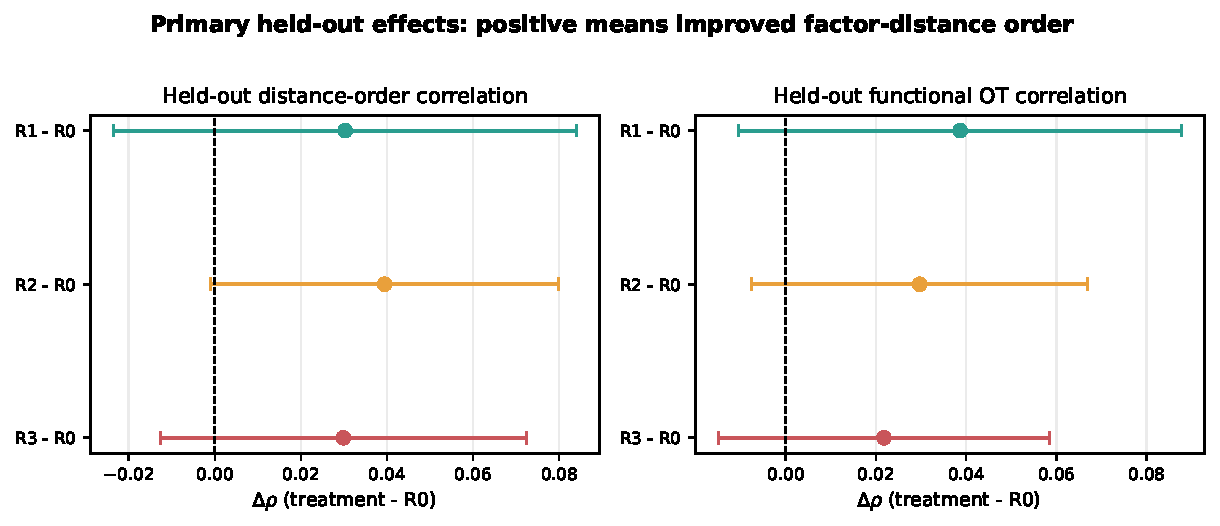
\includegraphics[width=0.96\textwidth]{figures/heldout_effect_forest.pdf}
\caption{Held-out Spearman effects relative to R0. All three constrained routers have positive mean effects, but every seed interval crosses zero. R3 therefore fails both primary held-out mediation gates.}
\label{fig:rho}
\end{figure}

For the primary R3--R0 contrast, held-out nominal $\rho$ changes by
\begin{equation}
 \Delta\rho_{\mathrm{nom}}=0.0299,
 \qquad 95\%\ \mathrm{CI}=[-0.0127,0.0725],
\end{equation}
and held-out functional $\rho$ changes by
\begin{equation}
 \Delta\rho_{\mathrm{func}}=0.0218,
 \qquad 95\%\ \mathrm{CI}=[-0.0148,0.0584].
\end{equation}
Four of five seeds are favorable in both cases, but the preregistered seed interval requirement is not met. R1 and R2 show the same pattern: positive means without a strictly positive interval.

\subsection{Stress improves, especially for R2}
\begin{figure}[H]
\centering
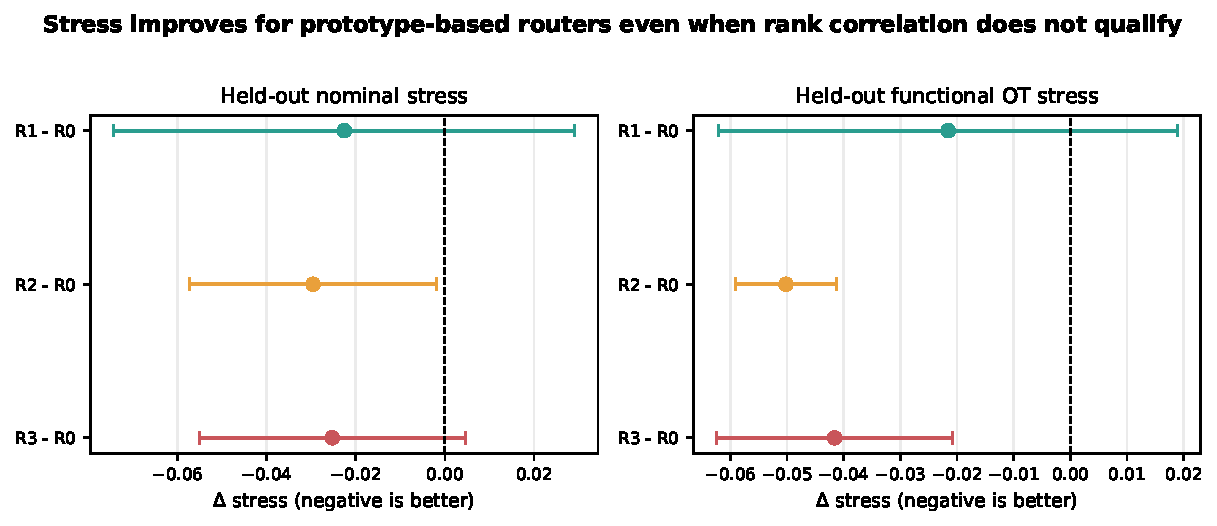
\includegraphics[width=0.96\textwidth]{figures/heldout_stress_forest.pdf}
\caption{Held-out stress effects relative to R0. Negative is better. R2 and R3 significantly reduce common-cost functional stress even though their distance-order correlations do not qualify.}
\label{fig:stress}
\end{figure}

R2 reduces held-out functional stress by $-0.0502$ with interval $[-0.0592,-0.0412]$; R3 reduces it by $-0.0416$ with interval $[-0.0624,-0.0208]$. Thus prototype-based routing produces a lower-distortion functional arrangement in an average metric sense, but not a sufficiently stable rank ordering across model seeds. R3 does not improve over R2: the R3--R2 held-out functional $\rho$ effect is $-0.0079$ with interval $[-0.0260,0.0101]$.

\begin{warningbox}[Reviewer interpretation]
A stress improvement should not be promoted to ``functional mediation passed.'' The gate was defined on held-out distance-order correlation, not stress alone. The correct statement is that prototype-based routing produces a reproducible reduction in functional metric distortion while failing the preregistered held-out rank-order criterion.
\end{warningbox}

\subsection{Prototype territories are too locally sharp}
\begin{figure}[H]
\centering
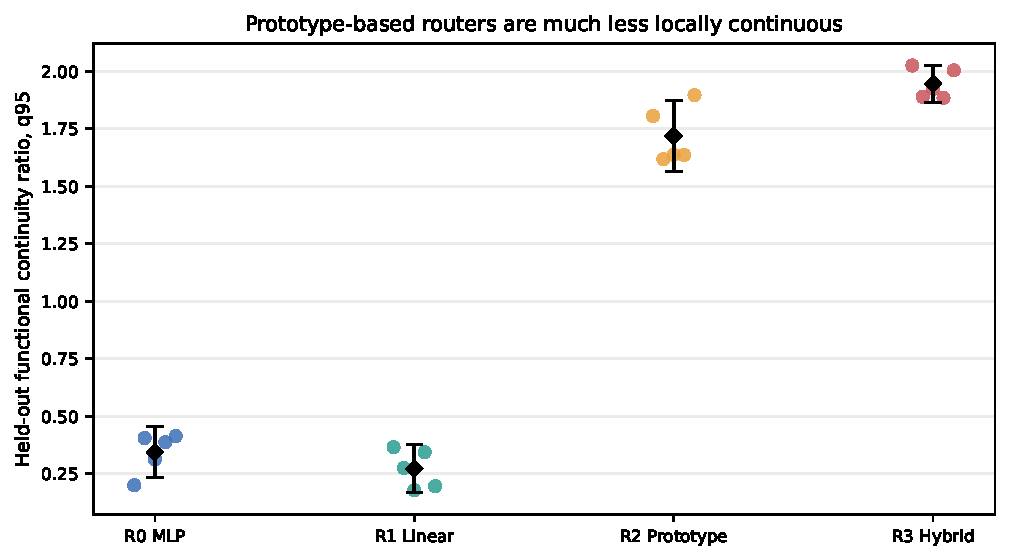
\includegraphics[width=0.78\textwidth]{figures/continuity_q95.pdf}
\caption{Held-out functional local-continuity q95 by seed. Diamonds show seed means with 95\% seed intervals; dots show individual seeds. Lower is smoother.}
\label{fig:continuity}
\end{figure}

Mean held-out functional q95 values are $0.344$ for R0, $0.271$ for R1, $1.718$ for R2, and $1.945$ for R3. The hybrid router is therefore approximately 5.7 times more sensitive than the MLP at the 95th percentile. The prototype component creates distinct territories, but the boundaries are too sharp for a continuity-qualified bridge.

Average host-territory specialization is $0.0024$ for R0, $0.0016$ for R1, $0.0470$ for R2, and $0.0534$ for R3. These values describe allocation concentration only. Because hosts are frozen and top-host ablations are not consistently more damaging than random controls, they do not establish learned functional specialization.

\subsection{Route-swap ordering passes}
\begin{figure}[H]
\centering
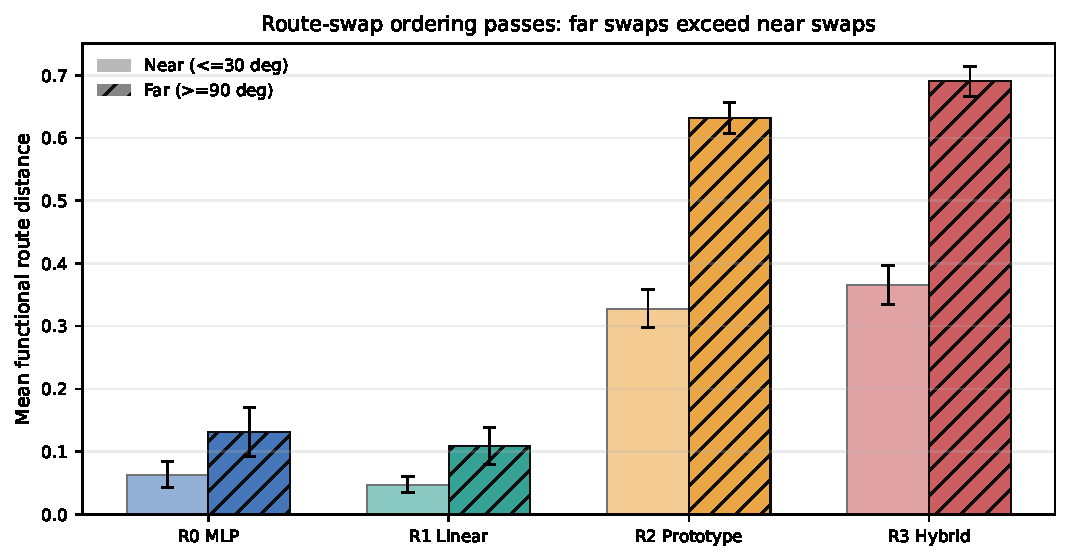
\includegraphics[width=0.82\textwidth]{figures/route_swap_order.pdf}
\caption{Mean common-cost route distance for near and far swaps. Error bars show standard deviation across five seeds. Far swaps exceed near swaps for every R3 seed, satisfying the preregistered route-swap-order gate.}
\label{fig:swap}
\end{figure}

Across seeds, R3 near swaps have mean functional distance $0.366$ and far swaps $0.691$. The corresponding values are $0.063$ and $0.131$ for R0, $0.047$ and $0.109$ for R1, and $0.328$ and $0.632$ for R2. This is the strongest positive v1.1.1 result: route positions associated with distant factors are functionally farther apart under the same frozen host metric.

The pass should still be interpreted narrowly. It shows ordered functional separation of existing routes, not that the router maps context to those routes continuously, causally, or with improved classification.

\subsection{Causal specificity fails and is seed-unstable}
\begin{figure}[H]
\centering
\includegraphics[width=0.82\textwidth]{figures/causal_csr.pdf}
\caption{Mean functional causal-specificity ratio by seed. The logarithmic scale exposes the unstable R1 outlier. The dashed line marks equality between tangent and orthogonal effects; the dotted line is the preregistered mean target.}
\label{fig:causal}
\end{figure}

R3 has mean functional CSR $0.897$ across seeds. Only seed 0 has a minimum source-bootstrap lower bound above one. R2 has two qualifying lower bounds but an across-seed mean below one. R1 exhibits three lower bounds above one, but its mean is dominated by a seed-4 ratio of $19.17$, indicating denominator instability rather than a qualified causal result. The preregistered R3 causal gate therefore fails.

Prediction-identity preservation passes: the mean of the per-seed minimum preservation rates is $0.981$ for R3. This indicates that the causal failure is not simply due to widespread class flips. Instead, tangent interventions are not reliably more functionally specific than matched orthogonal directions.

\subsection{Context reconstructs routes, but prototype mappings are less smooth}
\begin{figure}[H]
\centering

\includegraphics[width=0.84\textwidth]{figures/probe_controls.pdf}
\caption{Low-capacity ridge-probe reconstruction of held-out root routes from context. Full-context reconstruction is strongest for R0 and R1; prototype-based mappings are harder to interpolate. Angle shuffling removes most predictive structure.}
\label{fig:probe}
\end{figure}

Full-context held-out root-route $R^2$ averages $0.993$ for R0, $0.998$ for R1, $0.907$ for R2, and $0.875$ for R3. Removing the estimated factor tangent lowers the scores, while angle shuffling reduces them close to zero. This confirms factor-sensitive dependence of route on context, but it does not override the failed continuity and causal gates. A route can be decodable from context while still being locally sharp or functionally misaligned.

\subsection{Operational non-degradation fails}
\begin{figure}[H]
\centering

\includegraphics[width=0.96\textwidth]{figures/operational_summary.pdf}
\caption{Operational outcomes with 95\% seed intervals. R0 retains the best held-out and final trained accuracy. R1--R3 show slightly lower forgetting, but the accuracy losses exceed the preregistered non-degradation margin.}
\label{fig:operational}
\end{figure}

\begin{table}[H]
\centering
\caption{Operational outcomes across five seeds. Accuracy and forgetting are proportions.}
\label{tab:operational}
\small
\begin{tabular}{@{}lccc@{}}
\toprule
Method & Held-out accuracy & Final trained accuracy & Mean forgetting \\
\midrule
R0 MLP & $0.5709$ $[0.5594,0.5825]$ & $0.6353$ $[0.6225,0.6481]$ & $0.00200$ $[0.00030,0.00371]$ \\
R1 linear & $0.5611$ $[0.5516,0.5706]$ & $0.6248$ $[0.6165,0.6330]$ & $0.00050$ $[0.00006,0.00094]$ \\
R2 prototype & $0.5539$ $[0.5363,0.5715]$ & $0.6186$ $[0.6071,0.6300]$ & $0.00050$ $[0.00006,0.00094]$ \\
R3 hybrid & $0.5606$ $[0.5506,0.5707]$ & $0.6154$ $[0.6062,0.6247]$ & $0.00056$ $[-0.00008,0.00120]$ \\
\bottomrule
\end{tabular}
\end{table}

Relative to R0, R3 changes held-out accuracy by $-0.0103$ with interval $[-0.0175,-0.0031]$ and final trained accuracy by $-0.0199$ with interval $[-0.0381,-0.0017]$. Mean forgetting improves by $-0.00144$ with interval $[-0.00262,-0.00025]$. The result exposes a stability--plasticity trade-off: sharper constrained routes reduce already-small forgetting but cost more accuracy than the allowed one-point margin.

\section{Why the hybrid router failed}
\subsection{Local territories and global direction did not combine additively}
The R3 energy was intended to combine the local territories of R2 with the global directionality of R1:
\begin{equation}
 E_h(c)=\alpha E_h^{\mathrm{prototype}}(c)-\beta a_h^\top c+b_h.
\end{equation}
The result indicates that the prototype component dominates local behavior. R3 is more specialized than R2 and slightly farther under swaps, but also less continuous, no more correlated with held-out factor distances, and less accurate. The two desirable inductive biases did not simply add; their interaction produced sharper boundaries without qualified causal alignment.

\subsection{A flexible MLP is not geometrically clean, but remains operationally useful}
R0 has the weakest territorial structure and the lowest route-swap distances, yet the best accuracy. This demonstrates that a router can solve the current classification objective without preserving the intended geometry. Conversely, geometric structure does not automatically improve the task. Geometry must therefore remain an evaluated mechanism rather than an assumed virtue.

\subsection{The linear router remains a first-class baseline}
R1 is the smoothest constrained router and has only 20 parameters. Its held-out nominal and functional mean effects are positive but non-qualifying. Its exploratory causal ratios are highly unstable, including one extreme seed. The appropriate conclusion is not that R1 has solved mediation, but that a simple global map is a stronger baseline than a prototype-heavy route and should remain in every next-stage comparison.

\section{Claims, non-claims, and reviewer wording}
\begin{table}[H]
\centering
\caption{Recommended claim language.}
\label{tab:claims}
\small
\begin{tabularx}{\textwidth}{@{}Y c Y@{}}
\toprule
Claim & Status & Reviewer-safe wording \\
\midrule
Protocol isolation & Supported & Context, hosts, readout, and functional metric were held common across router treatments. \\
Held-out nominal mediation & Not established & Mean effects were positive, but seed intervals included zero. \\
Held-out functional mediation & Not established & Common-cost functional correlation did not meet the preregistered interval gate. \\
Functional metric distortion & Supported, secondary & R2 and R3 reduced held-out functional stress relative to R0. \\
Local continuity & Refuted for current R3 & Prototype-based maps had substantially heavier sensitivity tails. \\
Route-function ordering & Candidate support & Far factor swaps produced larger functional changes than near swaps in all R3 seeds. \\
Causal specificity & Not established & Tangent effects were not reliably greater than orthogonal controls. \\
Mature host specialization & Not tested & Hosts were frozen; only route allocation patterns and fixed-host ablations were measured. \\
Operational non-degradation & Refuted at margin & Accuracy losses exceeded the one-point equivalence margin. \\
Operational superiority & Not claimed & No accuracy, retention, cost, or robustness superiority was demonstrated. \\
\bottomrule
\end{tabularx}
\end{table}

\begin{plainbox}[Reviewer-facing central statement]
Geometry-MMALS G1 v1.1.1 completed a five-seed bridge-isolation pilot in which the sensory encoder, context encoder, host bank, synthesis layer, classifier, and functional host-cost matrix were held common across router treatments. The protocol-integrity gates passed. The hybrid directional-prototype router showed small positive but non-robust held-out geometry effects, reduced functional stress, failed continuity, causal-specificity, and operational-equivalence gates, and therefore did not qualify. Route-swap ordering and prediction-identity preservation passed, indicating non-arbitrary functional structure in the frozen routing ecosystem without establishing a complete or useful context-to-function bridge.
\end{plainbox}

\section{Recommended next experiment}
\subsection{Do not scale the present R3 to ten seeds}
The principal failure is not insufficient replication. The five-seed intervals already identify a mechanism problem: R3 is too sharp, not sufficiently causally aligned, and operationally costly. A ten-seed qualification of the same architecture would spend compute to refine a negative estimate rather than test a repaired hypothesis.

\subsection{Continuity-controlled simplex residual router}
The immediate next treatment should retain the common bank and common cost matrix while replacing the full hybrid energy with a small, bounded residual on a linear base:
\begin{align}
 \ell_h^{\mathrm{base}}(c)&=w_h^\top c+b_h,\\
 \delta_h^{\mathrm{proto}}(c)&=-\gamma_h\frac{d_C(c,\mu_h)^2}{2\sigma_h^2},\\
 r_h(c)&=\softmax_h\!\left(\ell_h^{\mathrm{base}}(c)+g(c)\,\delta_h^{\mathrm{proto}}(c)\right),
\end{align}
where $g(c)\in[0,g_{\max}]$ is a small gate initialized near zero. This makes the linear route the default and permits local prototype corrections only when supported by data.

A local simplex-continuity penalty should be preregistered:
\begin{equation}
 \loss_{\mathrm{cont}}=
 \E_{(a,b)\in\mathcal N}
 \left[\max\left(0,
 d_R(r_a,r_b)-\kappa d_C(c_a,c_b)
 \right)^2\right],
\end{equation}
with a matched-control treatment using the same parameter count but no continuity term. Both root-chord and Fisher--Rao route distances should be reported, while common-cost OT remains the primary functional metric.

\subsection{Revised evidence sequence}
\begin{enumerate}
\item \textbf{Immediate bridge repair:} smooth simplex residual, local continuity, common frozen hosts, R0/R1/R2/R3 retained as controls.
\item \textbf{Covariance/SPD stage:} only after the route map is continuous, test whether covariance geometry improves drift detection or uncertainty calibration.
\item \textbf{Route-function memory transport:} compare distributions of functional route states through time, not merely static factor routes.
\item \textbf{Adaptive host specialization:} unfreeze hosts selectively and test contribution, ablation, swap, recovery, and cross-seed specialization.
\item \textbf{Bottom-up host feedback and TPUT:} add host confidence, novelty, capacity, memory risk, and goal-conditioned future control only after the static bridge is qualified.
\end{enumerate}

\section{Limitations}
\begin{itemize}
\item The pilot is limited to RotatedMNIST, five model seeds, and a reduced training budget.
\item The context checkpoint is reproduced rather than loaded from one immutable external artifact; hashes provide within-run traceability.
\item The common host bank is built under uniform routing, which may create insufficient functional differentiation for later routing benefits.
\item The primary geometry gate uses Spearman distance-order correlation; stress reveals secondary structure not captured by the gate.
\item CSR ratios can be unstable when orthogonal effects are very small, as illustrated by R1 seed 4.
\item The execution notebook contained temporary import/configuration hotfixes and a stale pre-execution claim-manifest status. These are archival issues, not changes to the numerical results; this report supersedes that stale wording.
\item No standard continual-learning baseline is re-run in v1.1.1 because this experiment isolates router mechanisms rather than benchmark superiority.
\end{itemize}

\section{Conclusion}
The strict bridge-isolation experiment narrows the Geometry-MMALS research question. A common context map and fixed host ecosystem can support ordered functional route differences: far route swaps are reliably more consequential than near swaps, and prototype-based routers reduce functional stress. However, the current hybrid directional-prototype router does not convert those relations into a smooth, causally specific, or operationally safe allocation rule. Its territories are too sharp, its held-out correlation effects are not robust across seeds, and its accuracy cost exceeds the preregistered margin.

This is a useful falsification rather than an inconclusive run. The experiment validates the isolation scaffold and identifies the next mechanism to test: a linear-first, continuity-controlled route on the probability simplex with only a bounded local prototype residual. Geometry remains central, but it must be earned through smoother functional control and operational value.

\appendix
\section{Exact primary effect table}
\begin{table}[H]
\centering
\caption{Held-out effects versus R0, with 95\% seed intervals. Negative stress effects are favorable.}
\small
\begin{tabular}{@{}llrrr@{}}
\toprule
Treatment & Metric & Mean & CI low & CI high \\
\midrule
R1--R0 & nominal $\rho$ & 0.0303 & -0.0235 & 0.0841 \\
R1--R0 & functional $\rho$ & 0.0387 & -0.0104 & 0.0877 \\
R1--R0 & nominal stress & -0.0226 & -0.0742 & 0.0291 \\
R1--R0 & functional stress & -0.0215 & -0.0620 & 0.0190 \\
R2--R0 & nominal $\rho$ & 0.0394 & -0.0009 & 0.0798 \\
R2--R0 & functional $\rho$ & 0.0297 & -0.0075 & 0.0670 \\
R2--R0 & nominal stress & -0.0296 & -0.0572 & -0.0019 \\
R2--R0 & functional stress & -0.0502 & -0.0592 & -0.0412 \\
R3--R0 & nominal $\rho$ & 0.0299 & -0.0127 & 0.0725 \\
R3--R0 & functional $\rho$ & 0.0218 & -0.0148 & 0.0584 \\
R3--R0 & nominal stress & -0.0253 & -0.0551 & 0.0046 \\
R3--R0 & functional stress & -0.0416 & -0.0624 & -0.0208 \\
\bottomrule
\end{tabular}
\end{table}

\section{Artifact and reproducibility note}
The numerical evidence is archived in the accompanying \texttt{v1\_1\_1} result bundle. It contains aggregate CSV files, per-seed traces, host-cost matrices, checkpoint hashes, staged evaluation, causal interventions, route swaps, continuity distributions, and gate summaries. The separate 44-page executed-notebook PDF records the full five-seed run and export sequence. This manuscript is the reviewer-facing interpretation; the executed notebook remains the immutable visual audit record.

\begin{thebibliography}{99}
\bibitem{harbonnier-v109}
G. Harbonnier. \emph{Geometry-MMALS G1 v1.0.9: Stationary Geometry Pilot}. Internal technical report, 2026.

\bibitem{harbonnier-v110}
G. Harbonnier. \emph{Geometry-MMALS G1 v1.1.0: Functional Routing Results and v1.1.1 Roadmap}. Internal technical report, 2026.

\bibitem{harbonnier-v111-exec}
G. Harbonnier. \emph{Geometry-MMALS G1 v1.1.1: Bridge Isolation Executed Notebook}. Execution archive, 44 pages, 2026.

\bibitem{frechet1957}
M. Fr\'echet. Sur la distance de deux lois de probabilit\'e. \emph{Annales de l'ISUP}, VI(3):183--198, 1957.

\bibitem{amari1998}
S.-I. Amari. Natural gradient works efficiently in learning. \emph{Neural Computation}, 10(2):251--276, 1998.

\bibitem{cuturi2013}
M. Cuturi. Sinkhorn distances: Lightspeed computation of optimal transport. In \emph{Advances in Neural Information Processing Systems 26}, 2013.

\bibitem{peyre2019}
G. Peyr\'e and M. Cuturi. Computational optimal transport. \emph{Foundations and Trends in Machine Learning}, 11(5--6):355--607, 2019.

\bibitem{parisi2019}
G. I. Parisi, R. Kemker, J. L. Part, C. Kanan, and S. Wermter. Continual lifelong learning with neural networks: A review. \emph{Neural Networks}, 113:54--71, 2019.

\bibitem{shazeer2017}
N. Shazeer et al. Outrageously large neural networks: The sparsely-gated mixture-of-experts layer. In \emph{International Conference on Learning Representations}, 2017.
\end{thebibliography}

\end{document}
